% Created 2020-02-10 Mon 11:48
% Intended LaTeX compiler: pdflatex
\documentclass[11pt]{article}
\usepackage[utf8]{inputenc}
\usepackage[T1]{fontenc}
\usepackage{graphicx}
\usepackage{grffile}
\usepackage{longtable}
\usepackage{wrapfig}
\usepackage{rotating}
\usepackage[normalem]{ulem}
\usepackage{amsmath}
\usepackage{textcomp}
\usepackage{amssymb}
\usepackage{capt-of}
\usepackage{hyperref}
\usepackage{listings}
\linespread{1.0}
\usepackage[left=1.5cm,right=1.5cm,top=1.5cm,bottom=1.5cm]{geometry}
\setlength{\parindent}{0in}
\setlength{\parskip}{0.15cm}
\author{eo shiru}
\date{\today}
\title{}
\hypersetup{
 pdfauthor={eo shiru},
 pdftitle={},
 pdfkeywords={},
 pdfsubject={},
 pdfcreator={Emacs 28.0.50 (Org mode 9.3)}, 
 pdflang={English}}
\begin{document}

\tableofcontents

Todo spaeter mehr sterne damit ueberschriften nicht so billo riesig

Well-Formed is Not Enough
A well-formed XML document is a document that conforms to the XML syntax rules, like:

it must begin with the XML declaration
it must have one unique root element
start-tags must have matching end-tags
elements are case sensitive
all elements must be closed
all elements must be properly nested
all attribute values must be quoted
entities must be used for special characters
Even if documents are well-formed they can still contain errors, and those errors can have serious consequences.

Think of the following situation: you order 5 gross of laser printers, instead of 5 laser printers. With XML Schemas, most of these errors can be caught by your validating software.

\section{Definition \& Facts}
\label{sec:org7b5ca9a}
\begin{itemize}
\item \textbf{eXtensible Markup Language (XML)}
\begin{itemize}
\item W3C Recommendation – Universal format for structured documents and data on the Web
\item XML is a simple meta-language for Markup language definition
\begin{itemize}
\item Enables a semi-structured data model \(\rightarrow\) Documents of one type can be structured differently
\item Enables self-description of data, i.e. XML documents can contain data and structure of that data (no separation of data-schema and specification as in databases)
\end{itemize}
\item 1996 Beginning of development, 1998 W3C adopts XML as recommendation
\item XML = 80\% of SGML’s possibilities, but only 20\% of SGML’s complexity
\item XML documents can (like HTML) be written in a simple way (ASCII) and transported equally simply (HTTP)
\end{itemize}
\item “The function of the markup in an XML document is to describe its \textbf{storage and logical structure} and to \textbf{associate attribute-value pairs with its logical structures}. XML provides a mechanism, the \textbf{document type declaration}, to define constraints on the logical structure and to support the use of predefined storage units.”
\item \textbf{Elements} - define the logical structure
\item \textbf{Attributes} - enable element association with additional information via name-value pairs
\item \textbf{XML Declaration} - information for interpretation of the logical structure by a parser
\end{itemize}

\section{Basics}
\label{sec:org2ae71bb}
\begin{itemize}
\item XML documents consist of the XML Declaration, elements and attributes, eg:
\end{itemize}
\lstset{breaklines=true,language=XML,label= ,caption= ,captionpos=b,numbers=none}
\begin{lstlisting}
<?xml version="1.0"?>
<order OrderID="10643">
  <item>
    <room id=“Room10"/>
    </item>
    <item>
      <room id=“Room11"/>
  </item>
  <OrderDate
      ts="2004-05-17T00:00:00"/>
  <price>248.00 EUR</price>
</order>
\end{lstlisting}
\begin{itemize}
\item a XML document is:
\begin{itemize}
\item \textbf{well-formed} if it compiles with all the XML rules
\begin{itemize}
\item all elements are closed eg <tag>Data</tag>
\item empty elements are closed with "/" eg <emptyElemt />
\item attribute values in quotes <element attribute="123">
\end{itemize}
\item \textbf{valid} if
\begin{itemize}
\item it is well formed and
\item document rules adhere to Document Type Definition or a Schema
\end{itemize}
\end{itemize}
\end{itemize}
A "well formed" XML document is not the same as a "valid" XML document.
A "valid" XML document must be well formed. In addition, it must conform to a document type definition. An XML document validated against a DTD or Schema is both "Well Formed" and "Valid".

\subsection{Elements}
\label{sec:org263125a}
\begin{itemize}
\item an \textbf{Element} has a \emph{Name}, \emph{Start-} and \emph{End-Tag} as well as \emph{Content}
\begin{itemize}
\item \textbf{Content}: unstructured (character data), structured, mixed or empty
\end{itemize}
\end{itemize}
\lstset{breaklines=true,language=XML,label= ,caption= ,captionpos=b,numbers=none}
\begin{lstlisting}
<?xml version="1.0" encoding="utf-8"?>
<Elemente>

  <Unstrukturiert>
    <! [CDATA[ Beliebige Zeichen &  > < //]]>
  </Unstrukturiert>

  <Strukturiert>
    <UnterElement>
      <UnterElement>...</UnterElement>
    </UnterElement>
  </Strukturiert>

  <Gemischt>
    Daten
    <UnterElement> Daten </UnterElement>
    Daten
  </Gemischt>

  <Leer></Leer> == <Leer/>

</Elemente>

\end{lstlisting}
\subsection{Attributes}
\label{sec:org5750325}
\begin{itemize}
\item an \textbf{Attribute} is a name-value pair
\begin{itemize}
\item value (for now) of type String
\item order of attributes is irrelevant
\end{itemize}
\item Element vs Attribute
\begin{itemize}
\item attribute serves the sole purpose of transporting element's metadata
\item compact notation, but inflexible - no nesting
\end{itemize}
\end{itemize}
\lstset{breaklines=true,language=XML,label= ,caption= ,captionpos=b,numbers=none}
\begin{lstlisting}
<?xml version="1.0" encoding="utf-8"?>
<Beispiel>
  <Element attribut="Wert" sprache="DE" Datum="01.01.2020" />
</Beispiel>
\end{lstlisting}
\subsection{XML Declaration}
\label{sec:orgb3148a8}
\begin{itemize}
\item provides instructions to the XML Processor (order is relevant!)
\begin{itemize}
\item version (optional) = XML Version used
\item encoding (mandatory) = encoding of the XML Document
\item standalone (optional) = "yes" means that there are no external Markup Declarations to process (apart from the document itself)
\end{itemize}
\item must occur at the beginning of the document
\item \textbf{XML Processor} = the programm that processes the XML document, ie a parser, and enable access to the content and structure of the XML document
\end{itemize}
\lstset{breaklines=true,language=XML,label= ,caption= ,captionpos=b,numbers=none}
\begin{lstlisting}
<?xml version="1.0" encoding="utf-8" standalone="yes"?>
<?xml encoding="ISO-2022-JP"?>
\end{lstlisting}
\section{Rules for Well-Formedness}
\label{sec:org5d20b97}
\begin{itemize}
\item XML documents have at least one element
\begin{itemize}
\item the first element is called "root"
\end{itemize}
\item start and end tags are in the same content
\begin{itemize}
\item right: \texttt{<parent><child></child></parent>}
\item wrong: \texttt{<parent><child></parent></child>}
\end{itemize}
\item each non-empty start-tag must have a corresponding end tag (case-sensitive)
\item naming conventions must be complied with
\begin{itemize}
\item names start with "\_" or letters and can contain numbers
\item not allowed are especially ":" and "=" in a name, as well as names starting with "xml"
\end{itemize}
\item formatting (white space) in text is taken into account
\item attribute names of an element are always unique
\end{itemize}
\section{Namespaces}
\label{sec:orgf96decc}
XML namespaces are used for providing uniquely named elements and attributes in an XML document. They are defined in a W3C recommendation. An XML instance may contain element or attribute names from more than one XML vocabulary. If each vocabulary is given a namespace, the ambiguity between identically named elements or attributes can be resolved.
A simple example would be to consider an XML instance that contained references to a customer and an ordered book. Both the customer element and the book element could have a child element named title. References to the title element would therefore be ambiguous; placing them in different namespaces would remove the ambiguity.

Namespace concept:
\begin{itemize}
\item qualify elements and attributes with an URI (URI “addresses“ the space of elements and attributes)
\item Namespace URI identifies resources, which contain the names of contexts (spaces) (doesn‘t have to exist)
\item Namespaces can be assigned prefixes (One or more prefixes as well as a default namespace/standard namespace)
\end{itemize}

Example:
\begin{itemize}
\item Namespace \texttt{NS1} contains the following names: title, description
\item Namespace \texttt{NS2} contains the following names: title, fname, lname
\end{itemize}

\(\rightarrow\) let the prefixes be NS1=„\url{http://example.org/Textdocument}“ and NS2=„urn:schema:person“
\begin{itemize}
\item then <NS1:title> and <NS2:title> can be differentiated
\end{itemize}
\lstset{breaklines=true,language=XML,label= ,caption= ,captionpos=b,numbers=none}
\begin{lstlisting}
<?xml version="1.0" encoding="utf-8"?>
<root xmlns="urn:StandardNamespace"
      xmlns:ns1="http://example.org/Textdokument" xmlns:ns2="urn:schema:person">
  <ns1:title>Buchtitel</ns1:title>
  <ns2:title>Graf von</ns2:title>
  <element>im Default-Namespace</element>
</root>
\end{lstlisting}
\begin{itemize}
\item namespace declarations
\begin{itemize}
\item one or more per element
\item children inherit all declarations from parents
\end{itemize}
\item namespace restrictions (qualified): element is assigned to a namespace, ie
\begin{itemize}
\item qualified: assignment via prefix
\item qualified: assignment via standard namespace
\end{itemize}
\end{itemize}

\lstset{breaklines=true,language=XML,label= ,caption= ,captionpos=b,numbers=none}
\begin{lstlisting}
<?xml version="1.0" encoding="utf-8"?>
<ns1:root xmlns:ns1="urn:schema:f">
  <ns1:title ns1:attribut="42">Buchtitel</ns1:title>
  <element attribut="42">Unqualified</element>
</ns1:root>
\end{lstlisting}
\begin{itemize}
\item qualified element above would be "root"
\item unqualified element would be "element"
\item attributes can be assigned namespaces but are often not in order to achieve higher reusability (metadata association to the element) at the attribute level
\end{itemize}
\section{Document Description}
\label{sec:org324b285}
\subsection{Document Type Declaration}
\label{sec:org27fdbbd}
Contains or points to markup declarations that provides a grammar for a class of documents. This grammar is known as a document type definition, or DTD (W3C).
\begin{itemize}
\item parser directive for DTD use
\end{itemize}
\subsection{Document Type Definition (DTD)}
\label{sec:org752da27}
Set of markup declarations included in or referenced by an XML document (W3C).
\begin{itemize}
\item grammar describing the structure of XML data
\end{itemize}

A document type definition (DTD) is a set of markup declarations that define a document type for a SGML-family markup language (GML, SGML, XML, HTML).
A DTD defines the valid building blocks of an XML document. It defines the document structure with a list of validated elements and attributes. A DTD can be declared inline inside an XML document, or as an external reference (Wiki).

\begin{center}
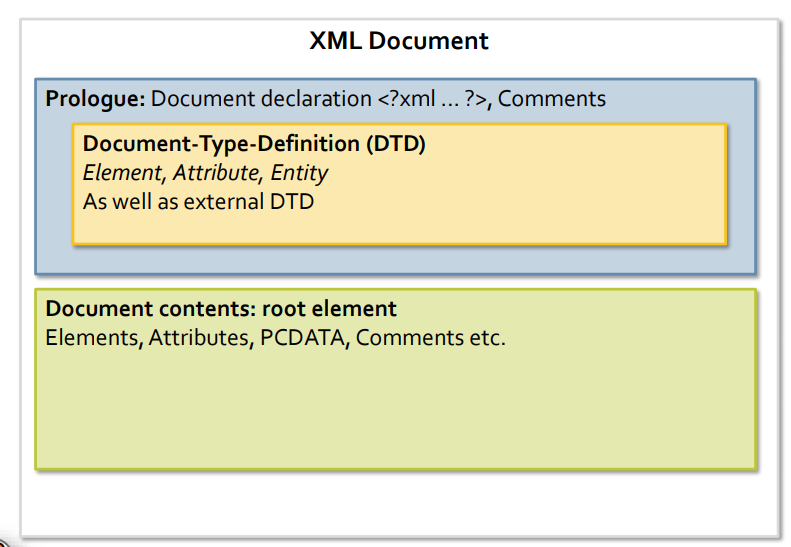
\includegraphics[width=240px]{./dtd.png}
\label{org8d8af9b}
\end{center}

\begin{itemize}
\item \texttt{<!DOCTYPE...>} specifies a DTD for the document which is either a grammar specification via URL or as a part of the document
\begin{itemize}
\item eg URL to an external DTD \texttt{<!DOCTYPE News System "http://example.org/news.dtd">}
\end{itemize}
\end{itemize}
\subsubsection{DTD - Grammar}
\label{sec:orgb43b643}
\begin{itemize}
\item \textbf{Document Type Definition}
\begin{itemize}
\item Doctypedecl ::= '<!DOCTYPE' S Name (S ExternalID)? S? ('[' (Markupdecl | DeclSep)* ']' S?)? '>‘
\item DeclSep ::= PEReference | S
\item Markupdecl ::= elementdecl | AttlistDecl | EntityDecl | NotationDecl | PI | Comment
\item example: <!ELEMENT recursion (item | (recursion, thing))>
\end{itemize}
\end{itemize}
\lstset{breaklines=true,language=XML,label= ,caption= ,captionpos=b,numbers=none}
\begin{lstlisting}
<recursion>
  <recursion>
    <recursion>
      <item/>
    </recursion>
    <thing/>
  </recursion>
  <thing/>
</recursion>
\end{lstlisting}

\begin{itemize}
\item there are 6 types of markup declaration: Element Type Declaration, Attribute-List Declaration, Entity Declaration, Notation Declaration, Processing Instruction, Comment
\item \textbf{Element Type Declaration}
\begin{itemize}
\item <!ELEMENT S Name S Content-Specification>
\item Content Specification
\begin{itemize}
\item any = arbitrary contents
\item emtpy = empty element
\item mixed = text and further subelements
\item children = sequence or set of subelements
\end{itemize}
\end{itemize}
\item \textbf{Attribute List Declaration}
\begin{itemize}
\item <!ATTLIST' S Name AttDef* S?>
\begin{itemize}
\item \emph{Name} is an element which attribute (list!) is bound to
\item AttDef defines name and type as well as value characteristics
\begin{itemize}
\item Types: eg CDATA (String), ID, IDREF, IDREFS, ENTITY, ENTITIES, NMTOKEN, NMTOKENS
\item possible value characteristics: \#REQUIRED, \#IMPLIED, \#FIXED value
\end{itemize}
\end{itemize}
\item example: <!ATTLIST elemname myenumtype (true|false|dontknow) 'true'> \(\rightarrow\) <elemname myenumtype="dontknow"/>
\item example: <!ATTLIST elem1 att2 CDAT \#REQUIRED> \(\rightarrow\) <elem1 att2="Value must be set here"/>
\item example: <!ATTLIST elem2 key ID \#IMPLIED> \(\rightarrow\) <elem2 key="a"/> having this element more than one time leads to an error
\end{itemize}
\end{itemize}
\subsubsection{DTD Advantages \& Disadvantages}
\label{sec:orgb3972ed}
\begin{itemize}
\item Advantages
\begin{itemize}
\item simple in writing (and understanding)
\item compact notation
\item Tool support
\end{itemize}
\item Disadvantages
\begin{itemize}
\item not an XML notation (double the learning curve)
\item poor expressivity (small number of data types, no name spaces)
\item little structuring possibilities
\end{itemize}
\end{itemize}
\subsection{Description with XML-Schema}
\label{sec:orga32848f}
\begin{itemize}
\item XML Schema Definition Language (XSD)
\begin{itemize}
\item since May 2001 a W3C recommendation
\item Motivation: "While XML 1.0 supplies a mechanism, the Document Type Definition (DTD) for declaring constraints on the use of markup, automated processing of XML documents requires more rigorous and comprehensive facilities in this area. Requirements are for constraints on how the component parts of an application fit together, the document structure, attributes, data-typing, and so on"
\end{itemize}
\item more possibilities such as: separation of tags and types, integration of concepts from object-orientation, inheritance, complex structures \& reuse, many data types, use of namespaces for use of more grammars, schema definition with full typing, documentation options
\item XML Schema entails all advantages of XML
\begin{itemize}
\item root element "schema"
\item element for description of elements are defined in the W3C namespace "XMLSchema" (Schema of all XML Schemas)
\end{itemize}
\item DTDs can be converted to XML Schemas (not the other way round)
\item Schmea definition in XML
\end{itemize}
\lstset{breaklines=true,language=XML,label= ,caption= ,captionpos=b,numbers=none}
\begin{lstlisting}
<?xml version="1.0" encoding="utf-8"?>
<xsd:schema
    targetNameSpace="http://example.org/Names"
    elementFormDefault="qualified"
    xmlns="http://example.org/Names"
    xmlns:xsd="http://www.w3.org/2001/XMLSchema">
</xsd:schema>
\end{lstlisting}
\begin{itemize}
\item the \texttt{targetNameSpace} attribute assigns a namespace to the vocabulary (elements, attributes etc)
\item if elements of an instance \emph{have to} belong to a namespace \texttt{elementFormDefault} is used as a validator directive (set to qualified)
\begin{itemize}
\item else defaults to "unqualified" which means an element is not checked for namespace alignment
\end{itemize}
\end{itemize}
\subsubsection{XML-Schema in Action}
\label{sec:orgb110357}
\begin{itemize}
\item schema instance = a creation of an XML document using a schema
\begin{itemize}
\item XML document, to which the targetNamespace of the XML schemas is assigned
\item the instance follows the schema rules, example:
\end{itemize}
\end{itemize}
\lstset{breaklines=true,language=XML,label= ,caption= ,captionpos=b,numbers=none}
\begin{lstlisting}
<?xml version="1.0" encoding="utf-8"?>
<News xmlns="http://example.org/news"
      xmlns:xsi="http://www.w3.org/2001/XMLSchema-instance"
      xsi:schemaLocation="http://example.org/new http://example.org/news.xsd">
  <Item>
    <date>10.10.2020</date>
    <description headline="Neues zu XML">XML macht Spass - und Gaedke..? fuck yo mama ;)</description>
  </Item>
</News>
\end{lstlisting}
\begin{itemize}
\item "News" (root element) is provided with a namespace
\begin{itemize}
\item namespace corresponds to the \texttt{targetNamespace} of the schema, which is bound via \texttt{schemaLocation}
\item \texttt{schemaLocation} forwards the XML processor where the schema to be used (URI: \ldots{}org/news) can be found (URL: \ldots{}org/news.xsd)
\end{itemize}
\end{itemize}
\begin{center}
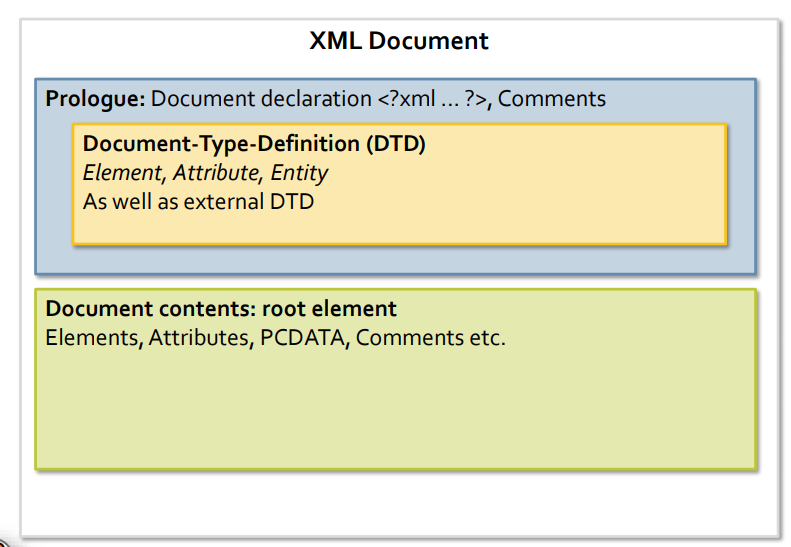
\includegraphics[width=.9\linewidth]{./dtd.png}
\end{center}
\begin{itemize}
\item in the example above the instance gets checked against the rules defined in the schema and the schema gets checked against the rules defined in the W3C-XML schema (\textbf{XML Instance Validation})
\end{itemize}
\end{document}
